\section{Условие задания}

Содержание проекта: Команда разработчиков из 16 человек занимается созданием карты города на основе собственного модуля отображения. Проект должен быть завершен в течение 6 месяцев. Бюджет проекта: 50 000 рублей.

\section{Задание 1}

В соответствии с первым заданием в проекте была произведена ликвидация перегрузки ресурсов при помощи автоматических параметров выравнивания. Автоматическое выравнивание работает следующим образом: задачи, в которых задействованы перегруженные ресурсы, смещаются, при этом первыми на выполнение ставятся критические задачи необходимые для успешного завершения проекта.

\begin{figure}[H]
    \centering
    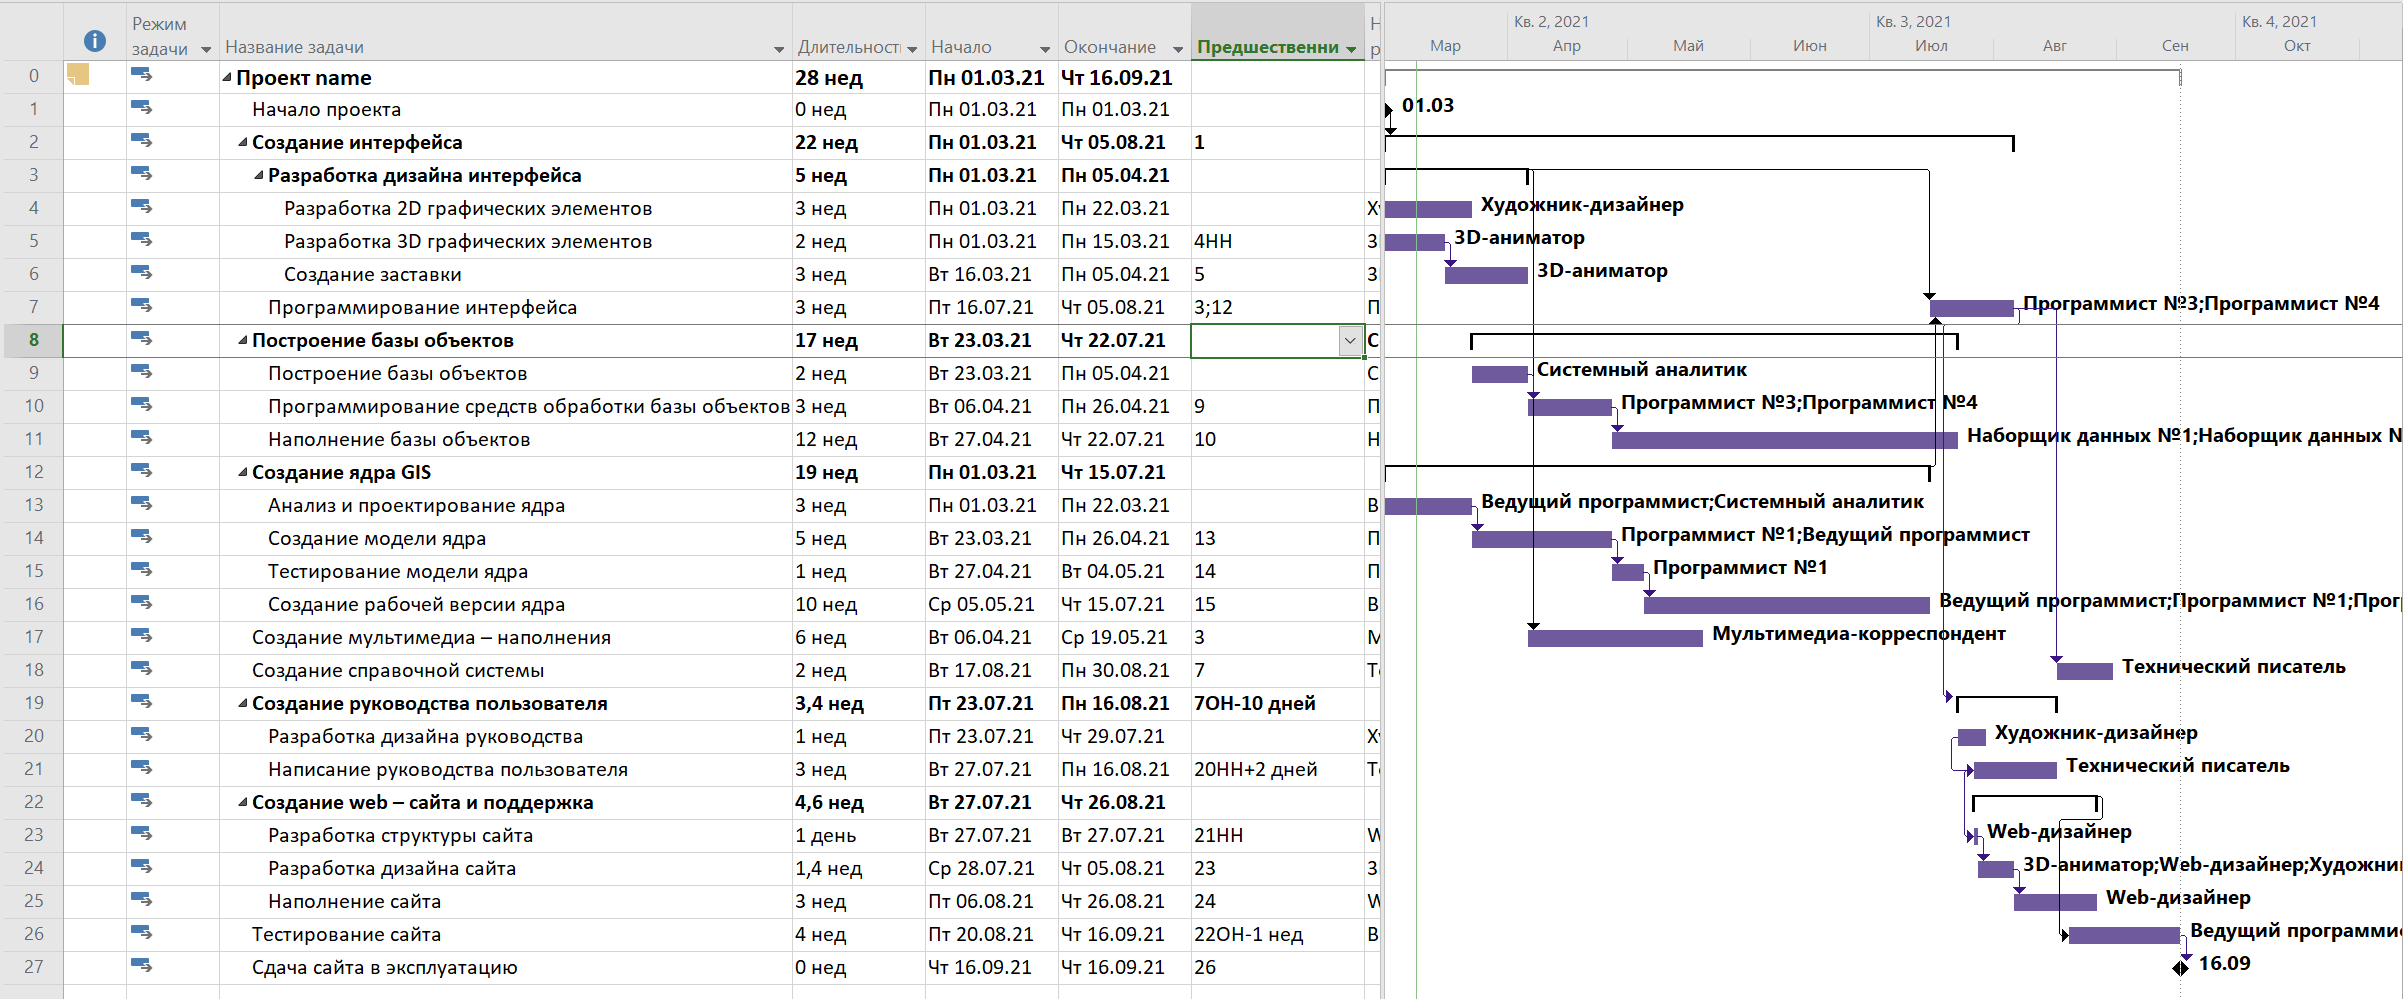
\includegraphics[width=0.8\textwidth]{img/content/task_1.png}
    \caption{Ликвидация перегрузки ресурсов в проекте}
    \label{fig:task_1}
\end{figure}

\section{Задание 2}

В план проекта было занесено проведение еженедельных совещаний по средам с 10 до 11 утра.

\begin{figure}[H]
    \centering
    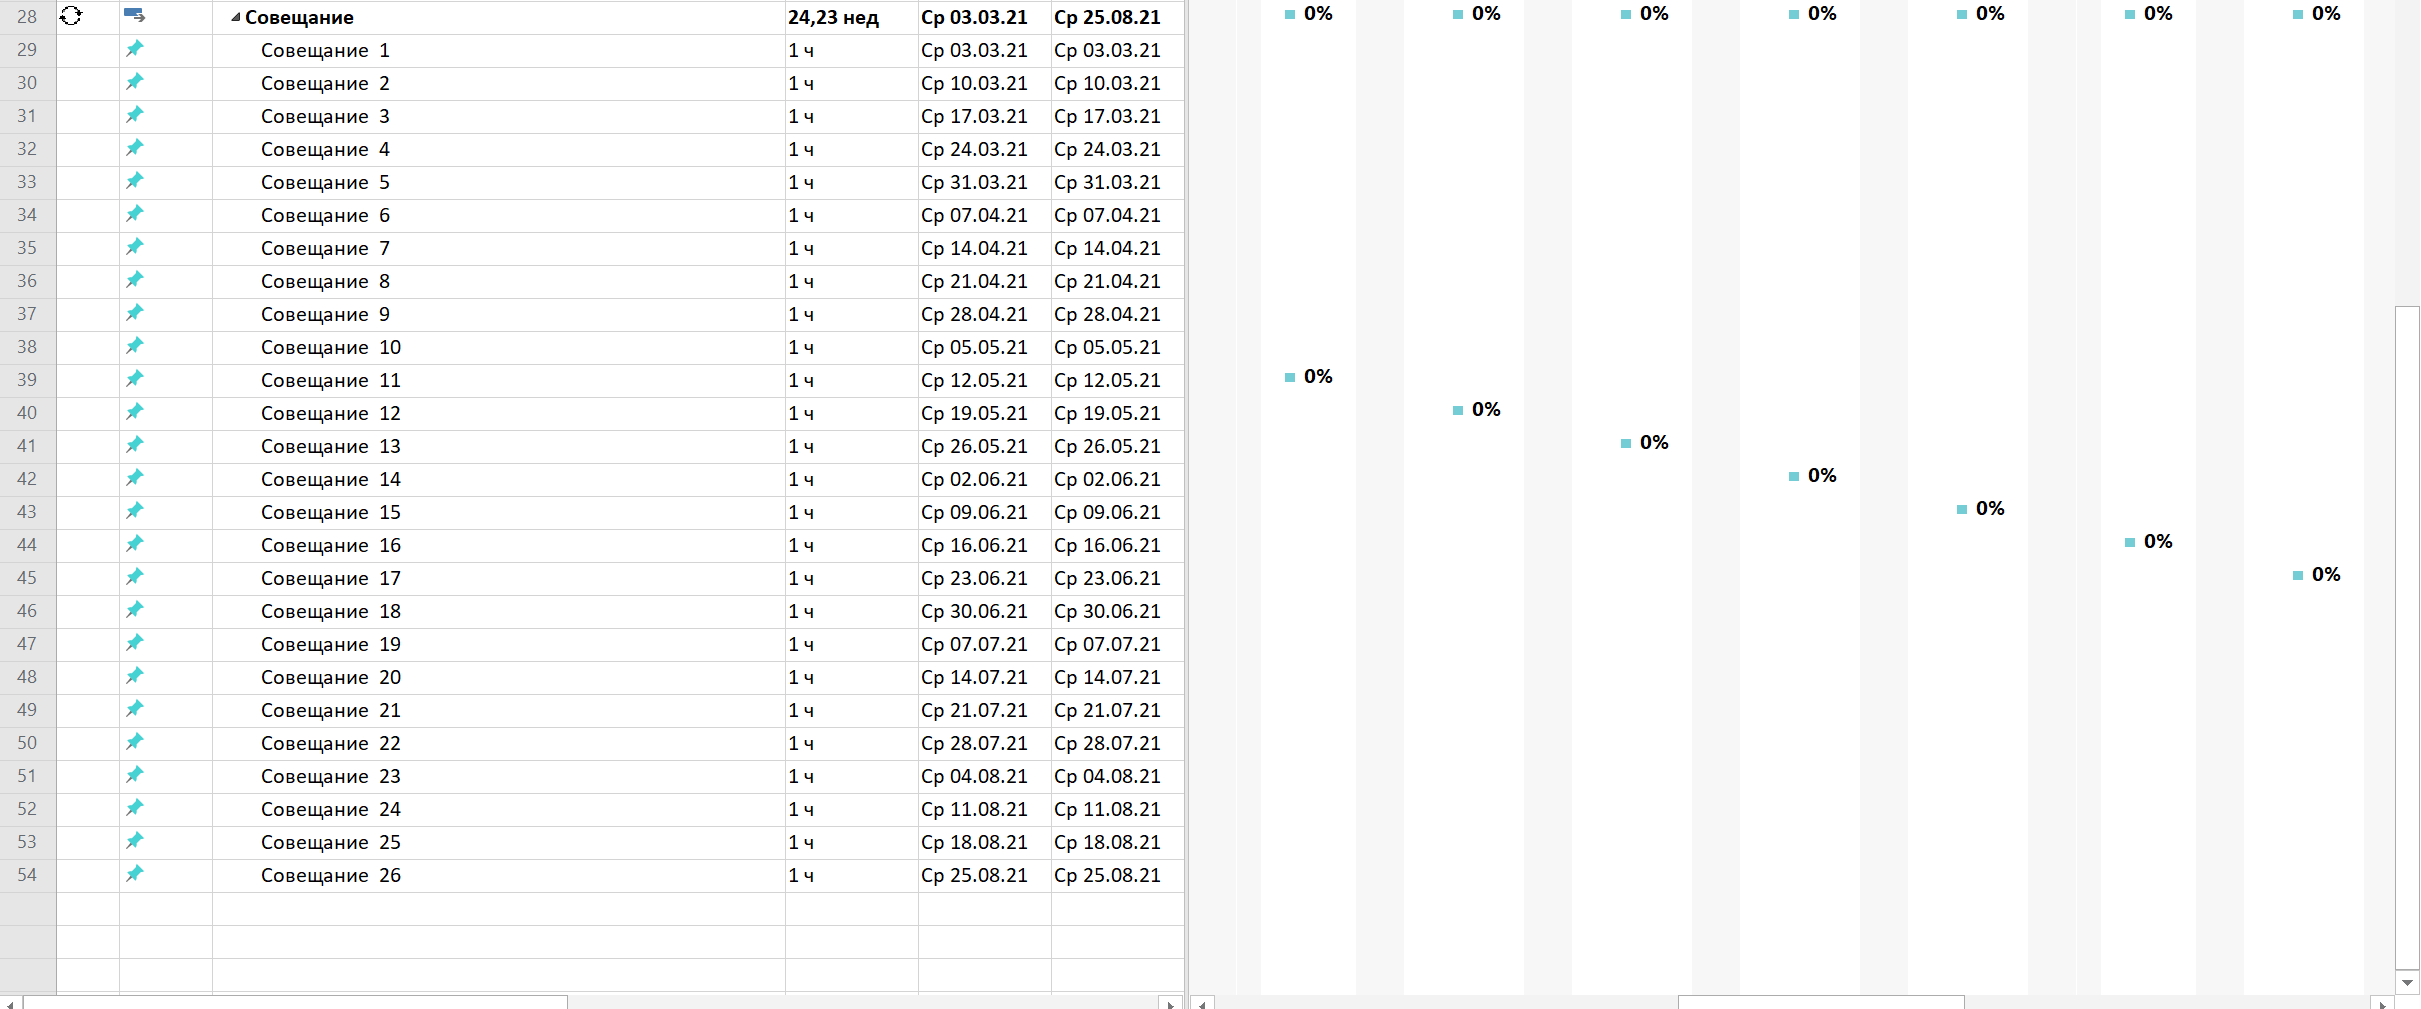
\includegraphics[width=0.8\textwidth]{img/content/task_2.png}
    \caption{Создание нового события с совещаниями}
    \label{fig:task_2}
\end{figure}

К совещанию были привлечены следующие ресурсы:

\begin{itemize}
    \item 3D-аниматор;
    \item Web-дизайнер;
    \item ведущий программист;
    \item мультимедиа-корреспондент;
    \item системный аналитик;
    \item технический писатель;
    \item художник-дизайнер.
\end{itemize}

\begin{figure}[H]
    \centering
    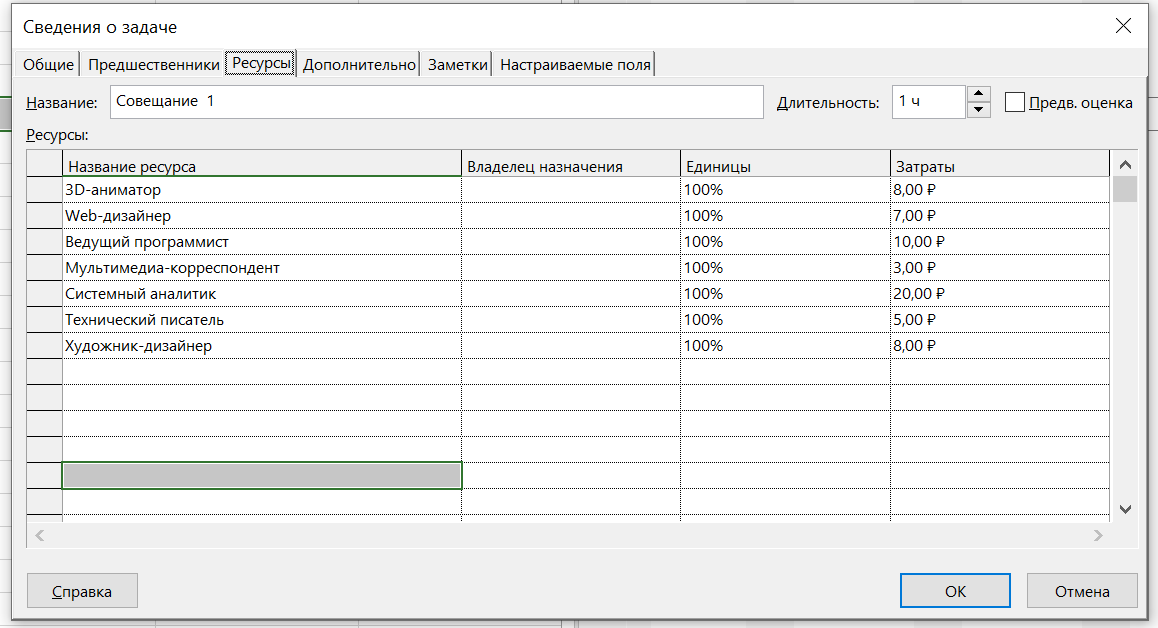
\includegraphics[width=0.8\textwidth]{img/content/task_2_resources.png}
    \caption{Привлечение ресурсов к совещанию}
    \label{fig:task_2_resources}
\end{figure}

После этого была устранена перегрузка ресурсов путем использования автоматического выравнивания использования ресурсов.

Также была проведена оптимизация финансовых параметров проекта (был добавлен дополнительный профиль в «листе ресурсов» для каждого ресурса, который использовался в случае проведения совещаний, – затраты в данном случае выставлялись равными 0).

\begin{figure}[H]
    \centering
    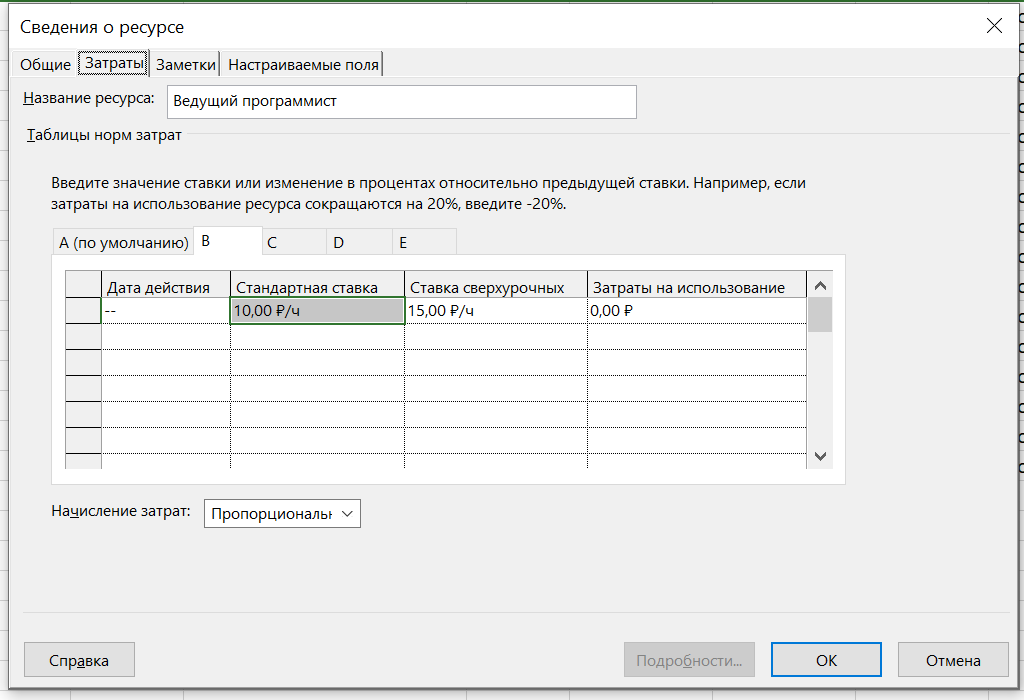
\includegraphics[width=0.8\textwidth]{img/content/task_2_resource_B.png}
    \caption{Оптимизация финансовых параметров проекта путем создания нового профиля}
    \label{fig:task_2_resource_B}
\end{figure}

После создания нового профиля с нулевыми затратами на использование в рамках совещаний было произведено изменение таблицы норм затрат на новый профиль для оптимизации финансовой составляющей проекта.

Проведенная оптимизация приведена ниже (затраты на проведение совещаний были уменьшены до 1 586 рублей).

\begin{figure}[H]
    \centering
    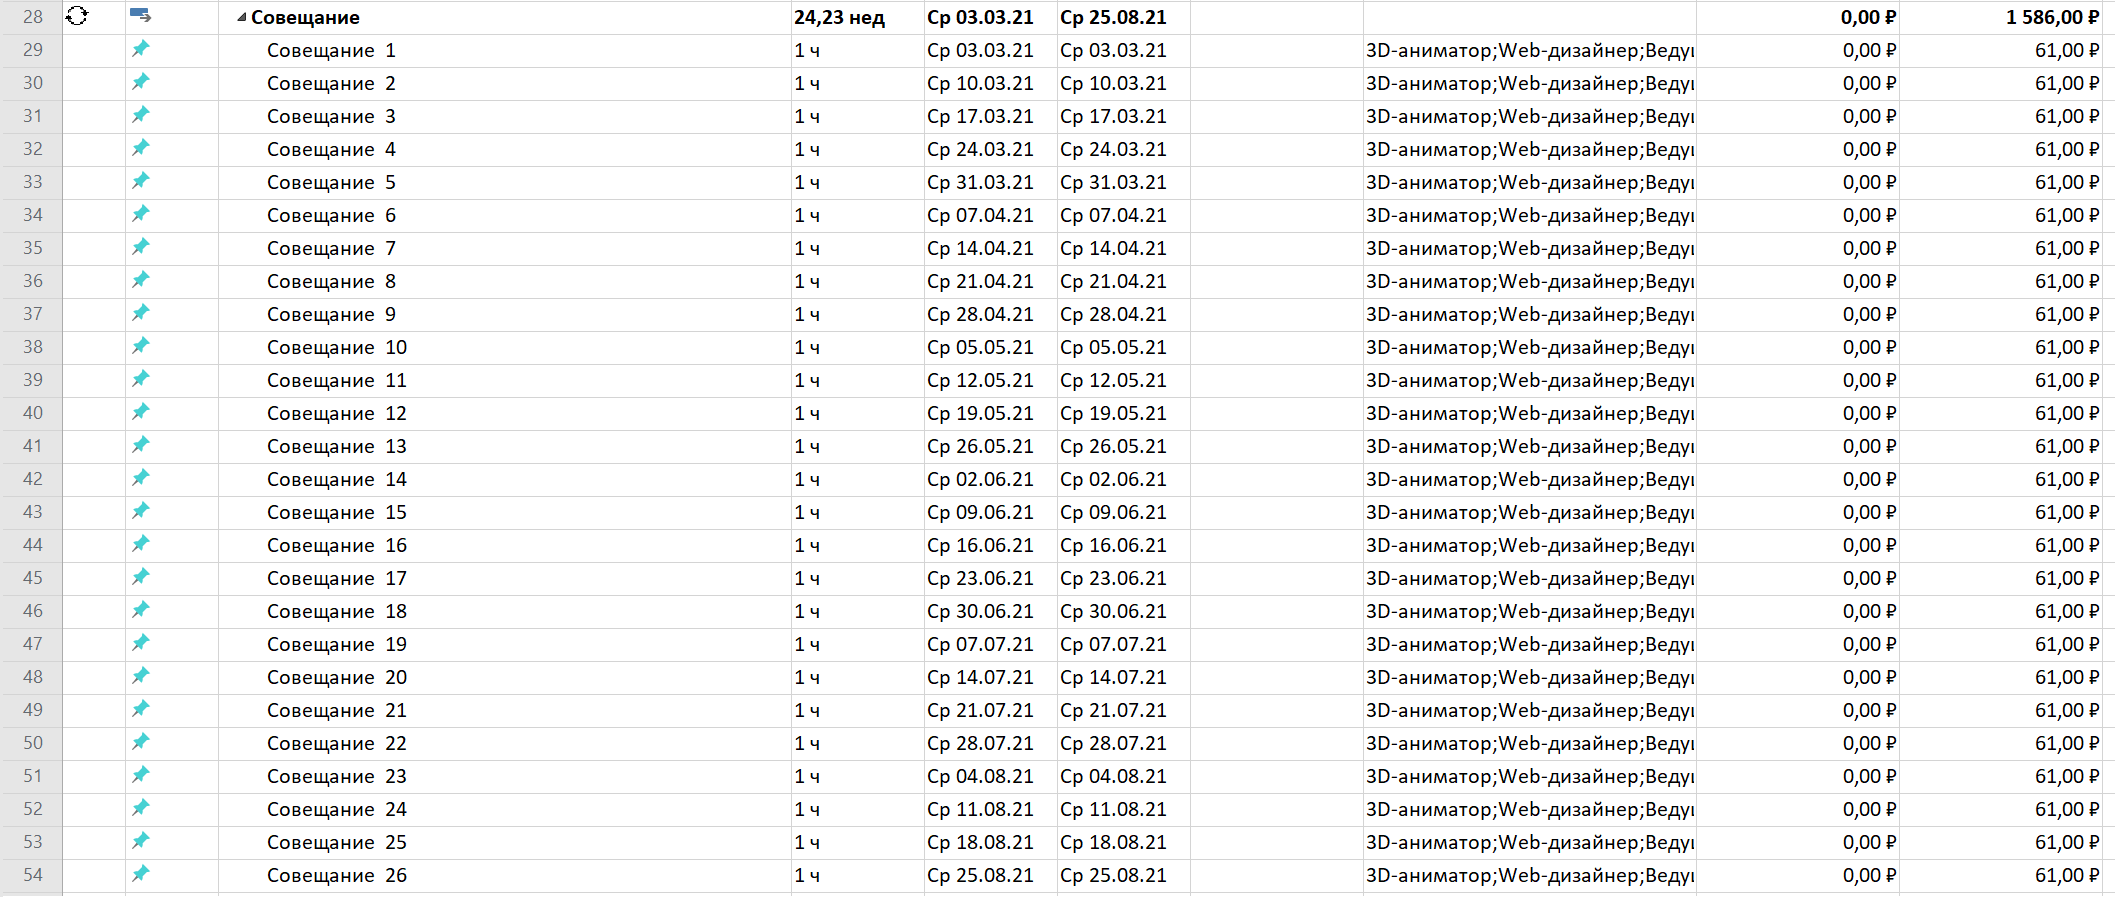
\includegraphics[width=0.8\textwidth]{img/content/task_2_meetings.png}
    \caption{Результат проведенной финансовой оптимизации проекта}
    \label{fig:task_2_meetings}
\end{figure}

\section{Задание 3}

На данный момент проект спланирован таким образом, что он завершается 16 сентября 2021 года.

Была произведена оптимизация критического пути следующими способами:

\begin{itemize}
    \item на все задачи, связанные с программированием (кроме «анализ и проектирование ядра») были задействованы все имеющиеся ресурсы этой сферы – задействовались программист №1, программист №2, программист №3, программист №4 и ведущий программист;
    \item в результате выполнения первого пункта было видно, что после выполнения последней важной задачи проекта – <<сдача сайта в эксплуатацию>> – совещания продолжали проводить, хотя в них не было надобности; все ненужные совещания были удалены (после 10 августа).
\end{itemize}

Общее состояние проекта после проведенной оптимизации показано ниже.

\begin{figure}[H]
    \centering
    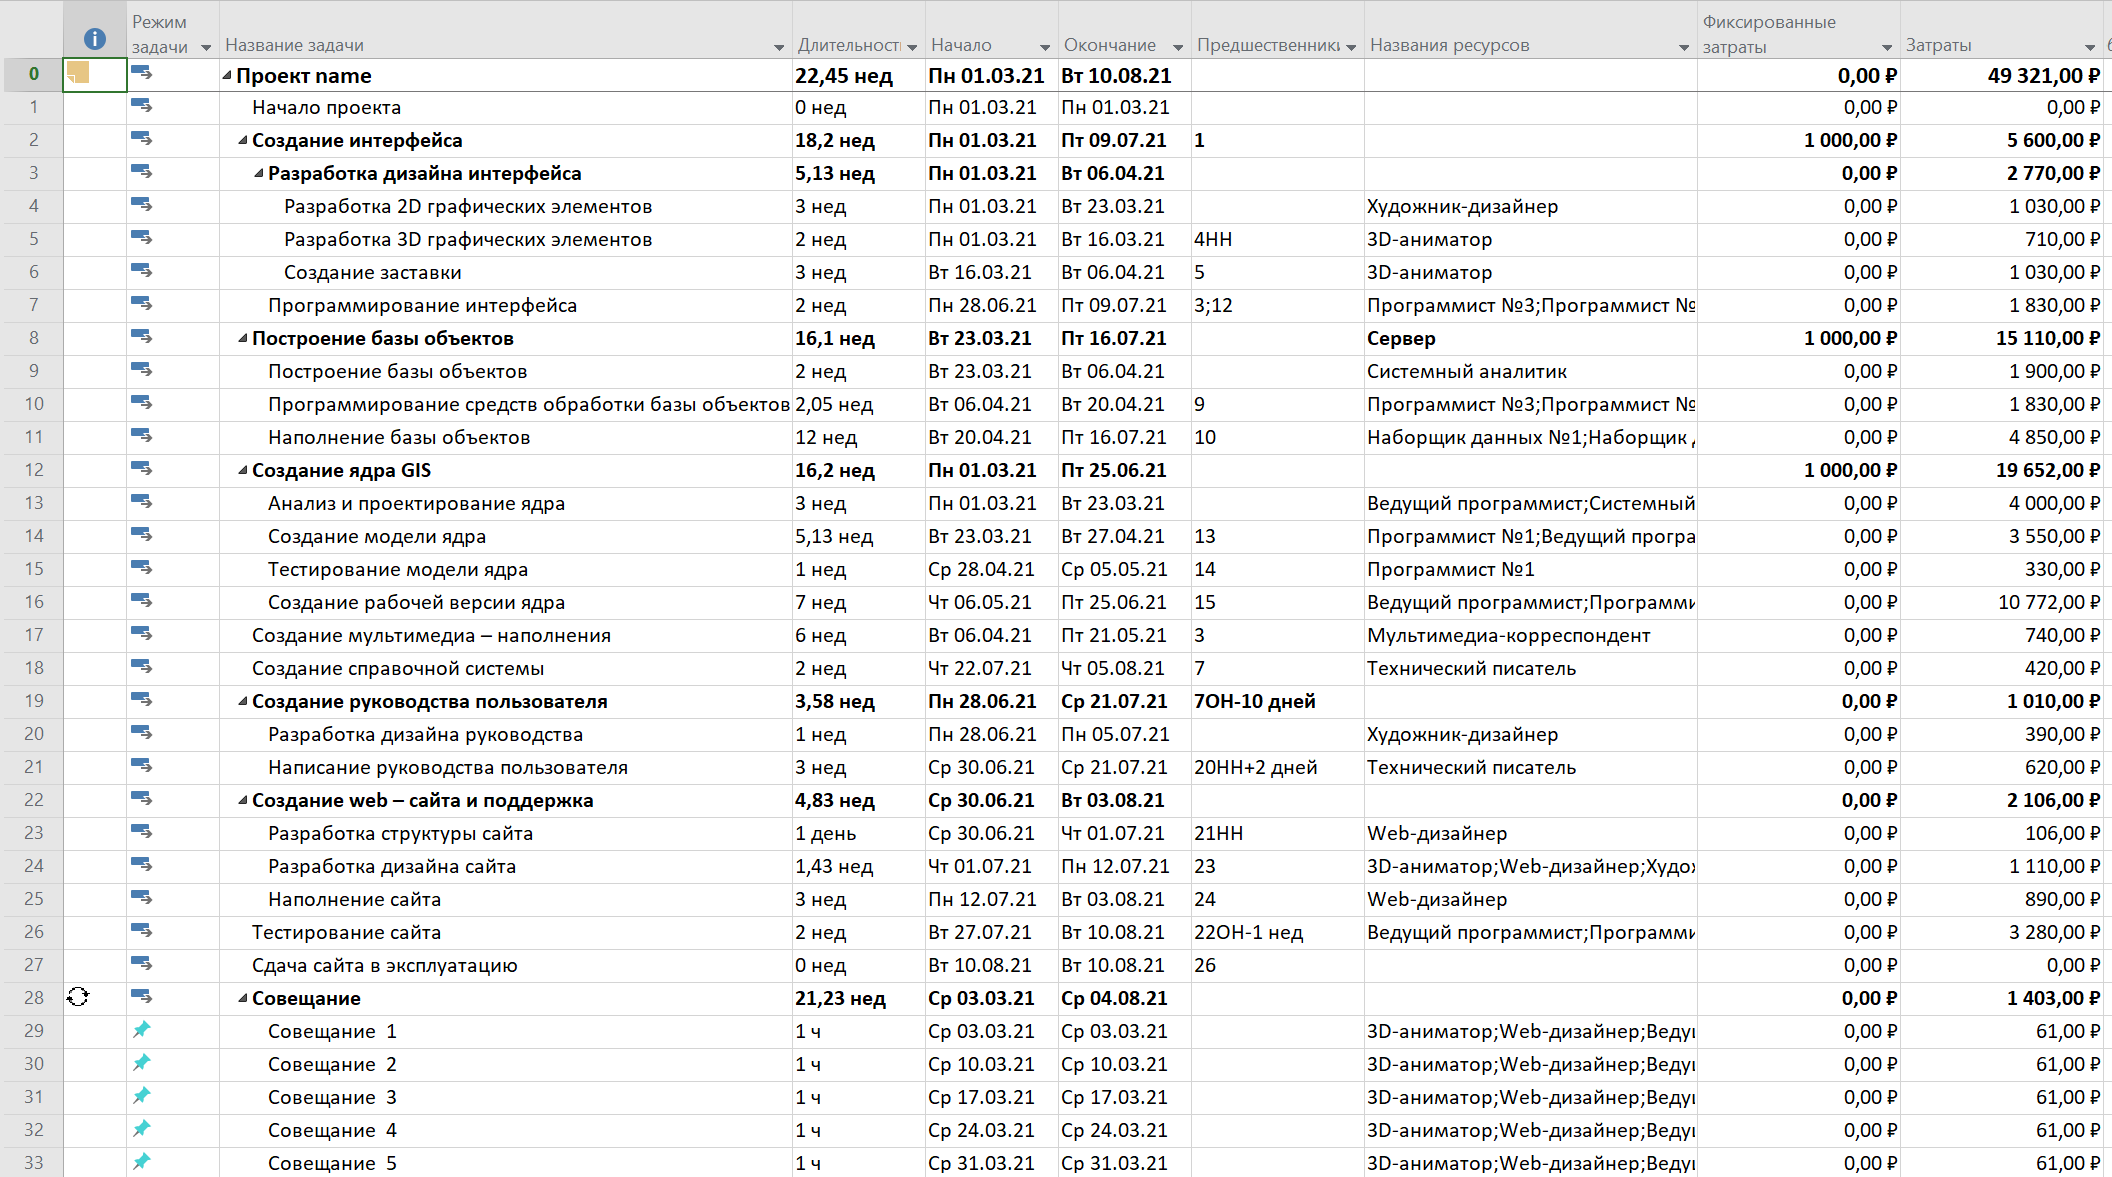
\includegraphics[width=0.8\textwidth]{img/content/task_3.png}
    \caption{Общее состояние проекта после проведенной оптимизации}
    \label{fig:task_3}
\end{figure}

Как можно заметить проект завершается 10 августа 2021 года, то есть длительность проекта равна 22.45 недель, а затраты составили 49 321 рублей.

Нижу можно увидеть диаграммы трудозатрат и затрат всех групп.

\begin{figure}[H]
    \centering
    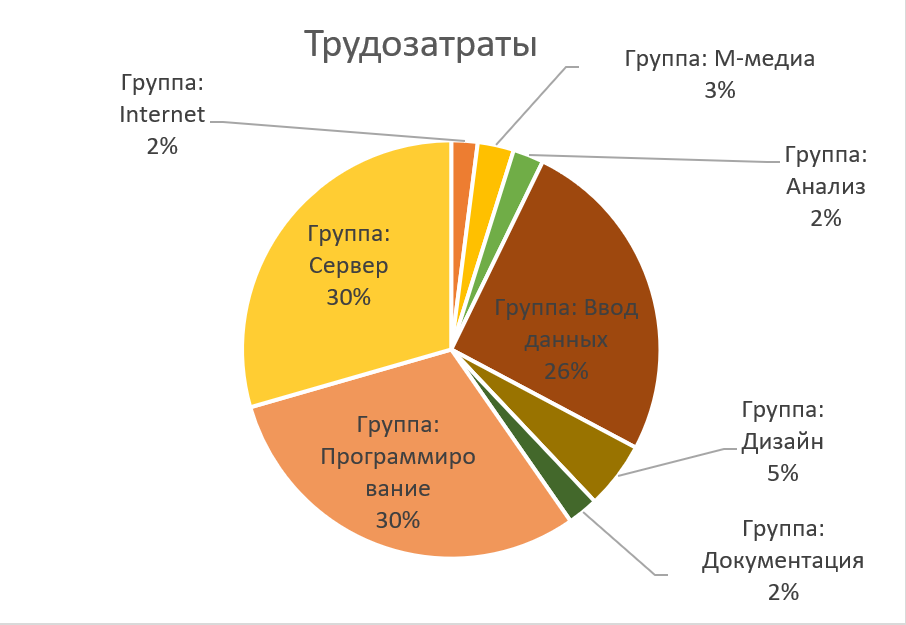
\includegraphics[width=0.8\textwidth]{img/content/diagram_hours.png}
    \caption{Трудозатраты}
    \label{fig:diagram_hours}
\end{figure}

\begin{figure}[H]
    \centering
    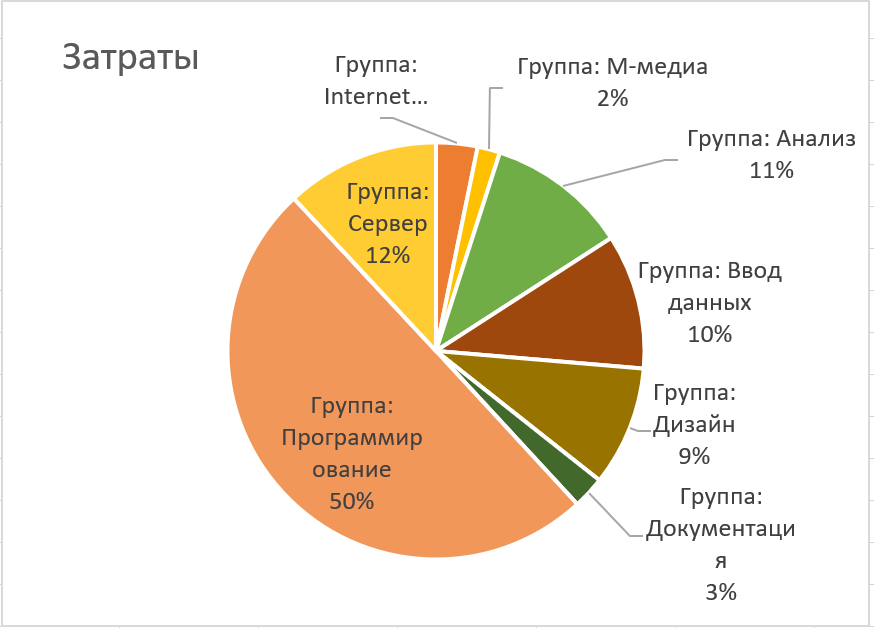
\includegraphics[width=0.8\textwidth]{img/content/diagram_money.png}
    \caption{Затраты}
    \label{fig:diagram_money}
\end{figure}

После получения приведенных выше диаграмм было произведено сохранение базового плана проекта через <<Проект>> -- <<Задать базовый план>>. Заданный базовый план задается для всего проекта

\begin{figure}[H]
    \centering
    
\includegraphics[width=0.8\textwidth]{img/content/task_3_finish.png}
    \caption{Задание базового плана}
    \label{fig:task_3_finish}
\end{figure}

\section{Вывод}

В ходе выполнения лабораторной работы №3 была изучена программа Microsoft Project 2019 и отработаны навыки ее использования для оптимизации временных и финансовых показателей проекта.

В результате была проведена успешная оптимизация проекта и было получено, что проект можно закончить 10 августа с бюджетом 49 321 рублей. Оптимизация была достигнута путем удаления лишних совещаний, выходящих за срок сдачи проекта, и перераспределением имеющихся ресурсов из группы <<Программирование>>. Статистика трудозатрат не изменилась после проведения данной оптимизации – самыми трудозатратными остались те же группы, что и во второй лабораторной работе. При этом наибольшие затраты бюджета составляет оплата работы программистов -- на них затрачено 50\% имеющегося бюджета.
